\subsection{YOLOv6 and YOLOv7}
\begin{frame}{}
    \LARGE Object Detection: \textbf{YOLOv6 and YOLOv7}
\end{frame}

\begin{frame}[allowframebreaks]{YOLOv6 and YOLOv7}
    \begin{figure}
        \centering
        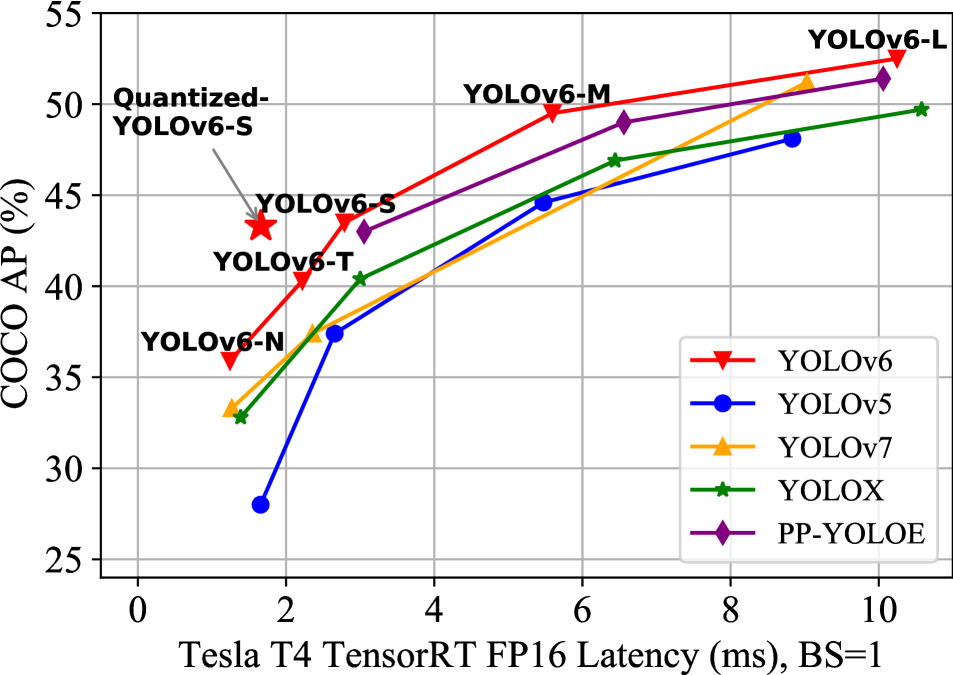
\includegraphics[width=1.0\textwidth,height=0.85\textheight,keepaspectratio]{images/object-detect/yolov6_ap_vs_latency.png}
        \caption*{\scriptsize Source: Li et al., ``YOLOv6: A Single-Stage Object Detection Framework for Industrial Applications'', arXiv:2209.02976, Fig.~1.}
    \end{figure}
\framebreak
    \textbf{YOLOv6 (2022) Highlights:}
    \begin{itemize}
        \item Released by Meituan with industrial deployment as the stated target, not by the original YOLO authors.
        \item \textbf{Anchor-free:} boxes are predicted from anchor points, so the hand-tuned anchor priors of v2--v5 are gone.
        \item \textbf{Backbone and neck:} EfficientRep for the small models, CSPStackRep blocks for the larger ones, with a Rep-PAN neck. Both re-parameterise into plain convolutions at inference time.
        \item \textbf{Head:} an efficient decoupled head, with Task Alignment Learning deciding which prediction is matched to which ground-truth box.
        \item \textbf{Losses:} VariFocal for classification, SIoU or GIoU for box regression, plus self-distillation on both tasks.
        \item \textbf{Performance:} YOLOv6-N reaches 35.9\% AP on COCO at 1234 FPS on a Tesla T4; YOLOv6-S 43.5\% AP at 495 FPS; YOLOv6-M/L 49.5\%/52.3\% AP.
    \end{itemize}
\framebreak
    \textbf{YOLOv7 (2022) Highlights:}
    \begin{itemize}
        \item From the YOLOv4 authors, built around \textit{trainable bag-of-freebies}: methods that cost training time but nothing at inference.
        \item \textbf{E-ELAN:} an extended layer-aggregation block that widens cardinality by expand, shuffle and merge, without disturbing the gradient path.
        \item \textbf{Compound scaling} for concatenation-based models, scaling block depth and transition width together so the two stay matched.
        \item \textbf{Planned re-parameterised convolution:} RepConv with its identity branch removed, so it can be placed alongside residual and concatenation connections.
        \item \textbf{Deep supervision:} an extra auxiliary head is trained on coarse labels assigned by the lead head, then dropped at inference.
        \item \textbf{Performance:} 56.8\% AP, the best of any real-time detector running at 30 FPS or more on a V100; YOLOv7-E6 gives 55.9\% AP at 56 FPS.
    \end{itemize}
\end{frame}
